\chapter{\textit{Pan troglodytes verus}}
\label{ch:chimp}

\begin{figure}[h!]
  \centering
    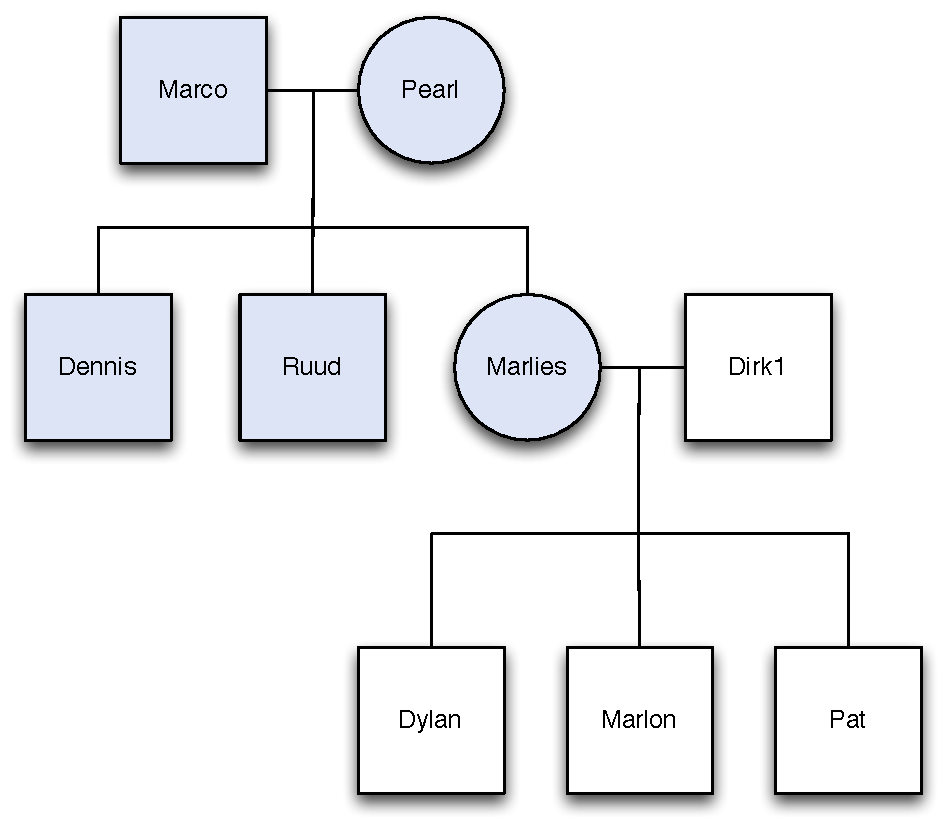
\includegraphics[width=0.7\textwidth]{pedigree}
  \caption{The three-generation chimpanzee pedigree.  The highlighted quintet is discussed in this chapter.  Average read coverage shown in parentheticals.}
  \label{fig:pedigree}
\end{figure}

\section{Introduction}

Finally, we briefly explore our software's technical limitations by touching on a second, previously analyzed dataset: a quintet taken from a three-generation, nine member pedigree of West African chimpanzees (\textit{Pan troglodytes verus}).  The processed samples are highlighted in Figure \ref{fig:pedigree}.  Venn {et al.} sequenced and examined this pedigree using reference-based methods for \textit{de novo} variation discovery, reporting a substantial paternal age effect to the overall mutation rate\cite{Venn:2014ep}.

In many ways, the chimpanzee quintet is a more computationally challenging dataset to process than the \textit{falciparum} crosses.  First, the genome is roughly two orders of magnitude larger; \textit{Plasmodium falciparum} is approximately $23$ Mbp, while \textit{Pan troglodytes} is $3,300$ Mbp ($3.3$ Gbp).  Second, the genome is diploid rather than haploid, an additional challenge during variant detection as now our software must contend with the presence of heterozygotes.  Third, we do not have draft-quality parental assemblies, and owing to the genome size, it is prohibitively expensive to generate such data.  We will be forced to rely solely on the Illumina data for the parents and children.  Fourth, the chimpanzee reference genome is reported to be of substantially lesser quality than the \textit{P. falciparum} reference, riddled with misassemblies and ambiguous sequence which can contribute to false negative and false positive variant calls\cite{Mallick:2009go}.  The chimpanzee assembly process employed a whole-genome shotgun sequencing approach yielding $5x$ coverage and $37,846$ supercontigs that were aligned to the human reference build to reconstruct the autosomes and sex chromosomes\cite{ChimpanzeeSequencingandAnalysisConsortium:2005fa}.  The \textit{falciparum} employed a whole-chromosome shotgun approach yielding approximately $14x$ coverage per chromosome.  With myriad gaps and errors in the chimpanzee reference sequence, a method unbiased towards the reference sequence should prove quite useful.  Finally, the coverage is substantially lower: $57x$ on average for the founders, $28x$ on average for the children, or one-half and one-third the coverage we had for samples in the previous chapter.

For precisely these reasons, the chimpanzee dataset is an important test-bed for our \textit{de novo} mutation calling software.  It permits a demonstration of our capacity to process much larger genomes than the \textit{falciparum} parasite.  Moreover, the problematic chimpanzee reference sequence and infeasibility of generating draft reference assemblies for the parents or children allow us to demonstrate the value of an approach that can leverage both, but requires neither.

\section{Data processing}

\subsection{Initial data}

We obtained the raw genomic sequencing data for the nine members of the pedigree.  For simplicity, we chose to focus our efforts on three children in the $F_1$ generation: Dennis, Ruud, and Marlies.  Their parents, Marco and Pearl, were sequenced to higher coverage.  This should give us greater confidence in our ability to distinguish novel kmers, kmers present in the child but absent from the parents, from those only absent from the parental genomes due to issues with sequencing.  The quintet is summarized in Table \ref{tbl:pedstats}.  All samples were sequenced on Illumina HiSeq $2000$ platforms using $100$ bp reads.

\begin{table}[]
\centering
\caption{Summary of \textit{P. troglodytes} quintet data}
\label{tbl:pedstats}
\begin{tabular}{@{}llllll@{}}
\toprule
                                       & Marco           & Pearl           & Dennis         & Ruud            & Marlies         \\ \midrule
Fragment size (bp)                     & $369 \pm 23$    & $399 \pm 31$    & $377 \pm 24$   & $415 \pm 27$    & $383 \pm 28$    \\
Coverage                               & $63 \pm 10$     & $57 \pm 8$      & $35 \pm 6$     & $22 \pm 3$      & $31 \pm 5$      \\
Cleaning threshold                     & $10$            & $9$             & $8$            & $4$             & $6$             \\
Kmers                                  &                 &                 &                &                 &                 \\
\multicolumn{1}{r}{\textit{dirty}}     & $7.7e9$         & $9.0e9$         & $5.9e9$        & $4.4e9$         & $5.2e9$         \\
\multicolumn{1}{r}{\textit{clean}}     & $2.6e9$         & $2.7e9$         & $2.5e9$        & $2.7e9$         & $2.6e9$         \\
Novel kmers                            &                 &                 &                &                 &                 \\
\multicolumn{1}{r}{\textit{initial}}   & -               & -               & $126,536$      & $348,374$       & $121,834$       \\
\multicolumn{1}{r}{\textit{final}}     & -               & -               & $33,535$       & $30,794$        & $20,923$        \\ \bottomrule
\end{tabular}
\end{table}

\subsection{Sample processing}

Precisely as we did for the \textit{P. falciparum} samples in the previous chapter, we used the available Illumina data to construct the de Bruijn graph structures for each child with McCortex, using a kmer size of $47$ bp and discarding bases with a quality score less than $Q5$.  McCortex's automatic cleaning algorithm was applied to the dirty graph for each sample.  We did not apply the paired-end read threading and contig emission steps as contigs were not required for our analysis.

\subsection{Novel kmers}

We produced a list of novel kmers per child in the manner described in Chapter \ref{ch:methods}, selecting kmers present in the cleaned graph of the child but absent in the dirty graphs of the parents ("initial" in Table \ref{tbl:pedstats}), then applying our filters described in Chapter \ref{ch:realdata} for coverage (set at $5x$ in this dataset), non-chimpanzee contamination\footnote{Examining the results of the contamination check, it is evident that some samples contain small numbers of kmers that BLAST identifies as coming from human (hundreds) or gorilla (dozens).  Given the evolutionary relationships between the three species, it is perhaps not unreasonable to allow these kmers into the analysis, as they may misattributed in the BLAST database.  Instead, we have opted to remain conservative and exclude these from consideration.}, orphan removal and over-cleaning detection.

\subsection{Additional filters for low-coverage data}

Given the excessively large number of novel kmers in the final sets (an order of magnitude larger than what we might expect assuming $50$ \textit{de novo} SNPs per sample, each generating $47$ novel kmers), we were concerned that the lower read depth on these samples could contribute to false positives \textit{de novo} mutations.  Lower coverage and the presence of heterozygotes (which will halve the coverage seen on each allele) should make it substantially more difficult for the McCortex software to automatically determine a suitable coverage threhold for kmers arising from sequencing error versus true genomic data.  This may result in evidence against a putative mutation being discarded.  Inspection of subgraphs associated with novel kmers revealed a number of kmers that had been erroneously and incompletely cleaned.

An example SNV found in the pedigree founders, Pearl and Marco, and $F_1$ progeny, Ruud, is shown in Figure \ref{fig:missingnovelkmersandtable}.  At first glance, this image seems to depict an $A/C$ heterozygote on the haplotypic background of the mother.  This is evident from the child's path (red) branching off from the mother and father (green and blue, respectively) at the top of the image and rejoining $47$ kmers later towards the bottom of the figure.  A child's path can also be seen tracking along the parental path between the two junctions, implying heterozygote status.  However, two elements of this plot are suspicious.  First, paternal edges are present outside the junctions, but absent within.  Second, many of the kmers in the alternate branch are not novel (as indicated by the grey circles rather than red).  Closer examination of each kmer in the alternate branch (we have highlighted one for clarity) reveals that while the parental edges $G$ and $A$ are absent in the dirty graph, they are absent in the clean graph.  By chance, two kmers had zero coverage in both the clean and dirty graphs, leading to the false-positive call.

\begin{figure}[h!]
  \centering
    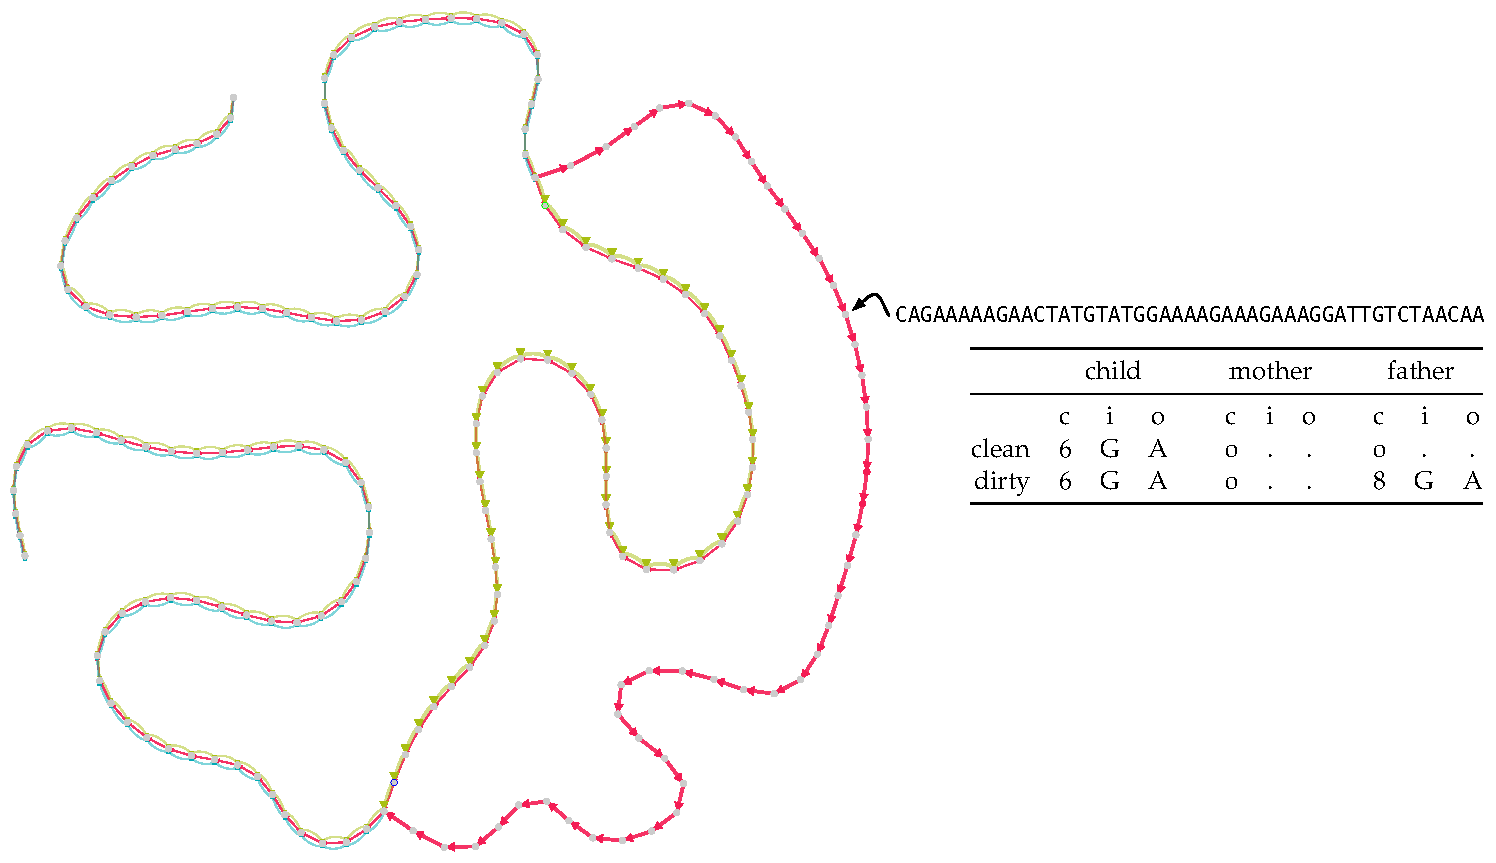
\includegraphics[width=0.9\textwidth]{missingnovelkmersandtable}
  \caption{A putative and suspicious \textit{de novo} SNP with very few novel kmers (filled red circles), and many non-novel kmers (filled grey circles) along the alternate branch.  An example kmer is highlighted; its coverage (c), incoming edges (i), and outgoing edges (o) are shown in the inset table.}
  \label{fig:missingnovelkmersandtable}
\end{figure}

%Gaps in the chimpanzee reference assembly may contribute to this peculiar behavior.  Figure \ref{fig:refhole} depicts read coverage in the aforementioned pedigree founders and F1 progeny.  The SNV depicted in the graph visualization above is shown to the left of this figure, while the assembly gap can be seen to the right.  Reads overlapping the gap may not align properly to this locus.  Additional variation on the same read proximate to the gap may not align at all, resulting in an allele-specific coverage drop out in the alignment data.
%
%\begin{figure}[h!]
%  \centering
%    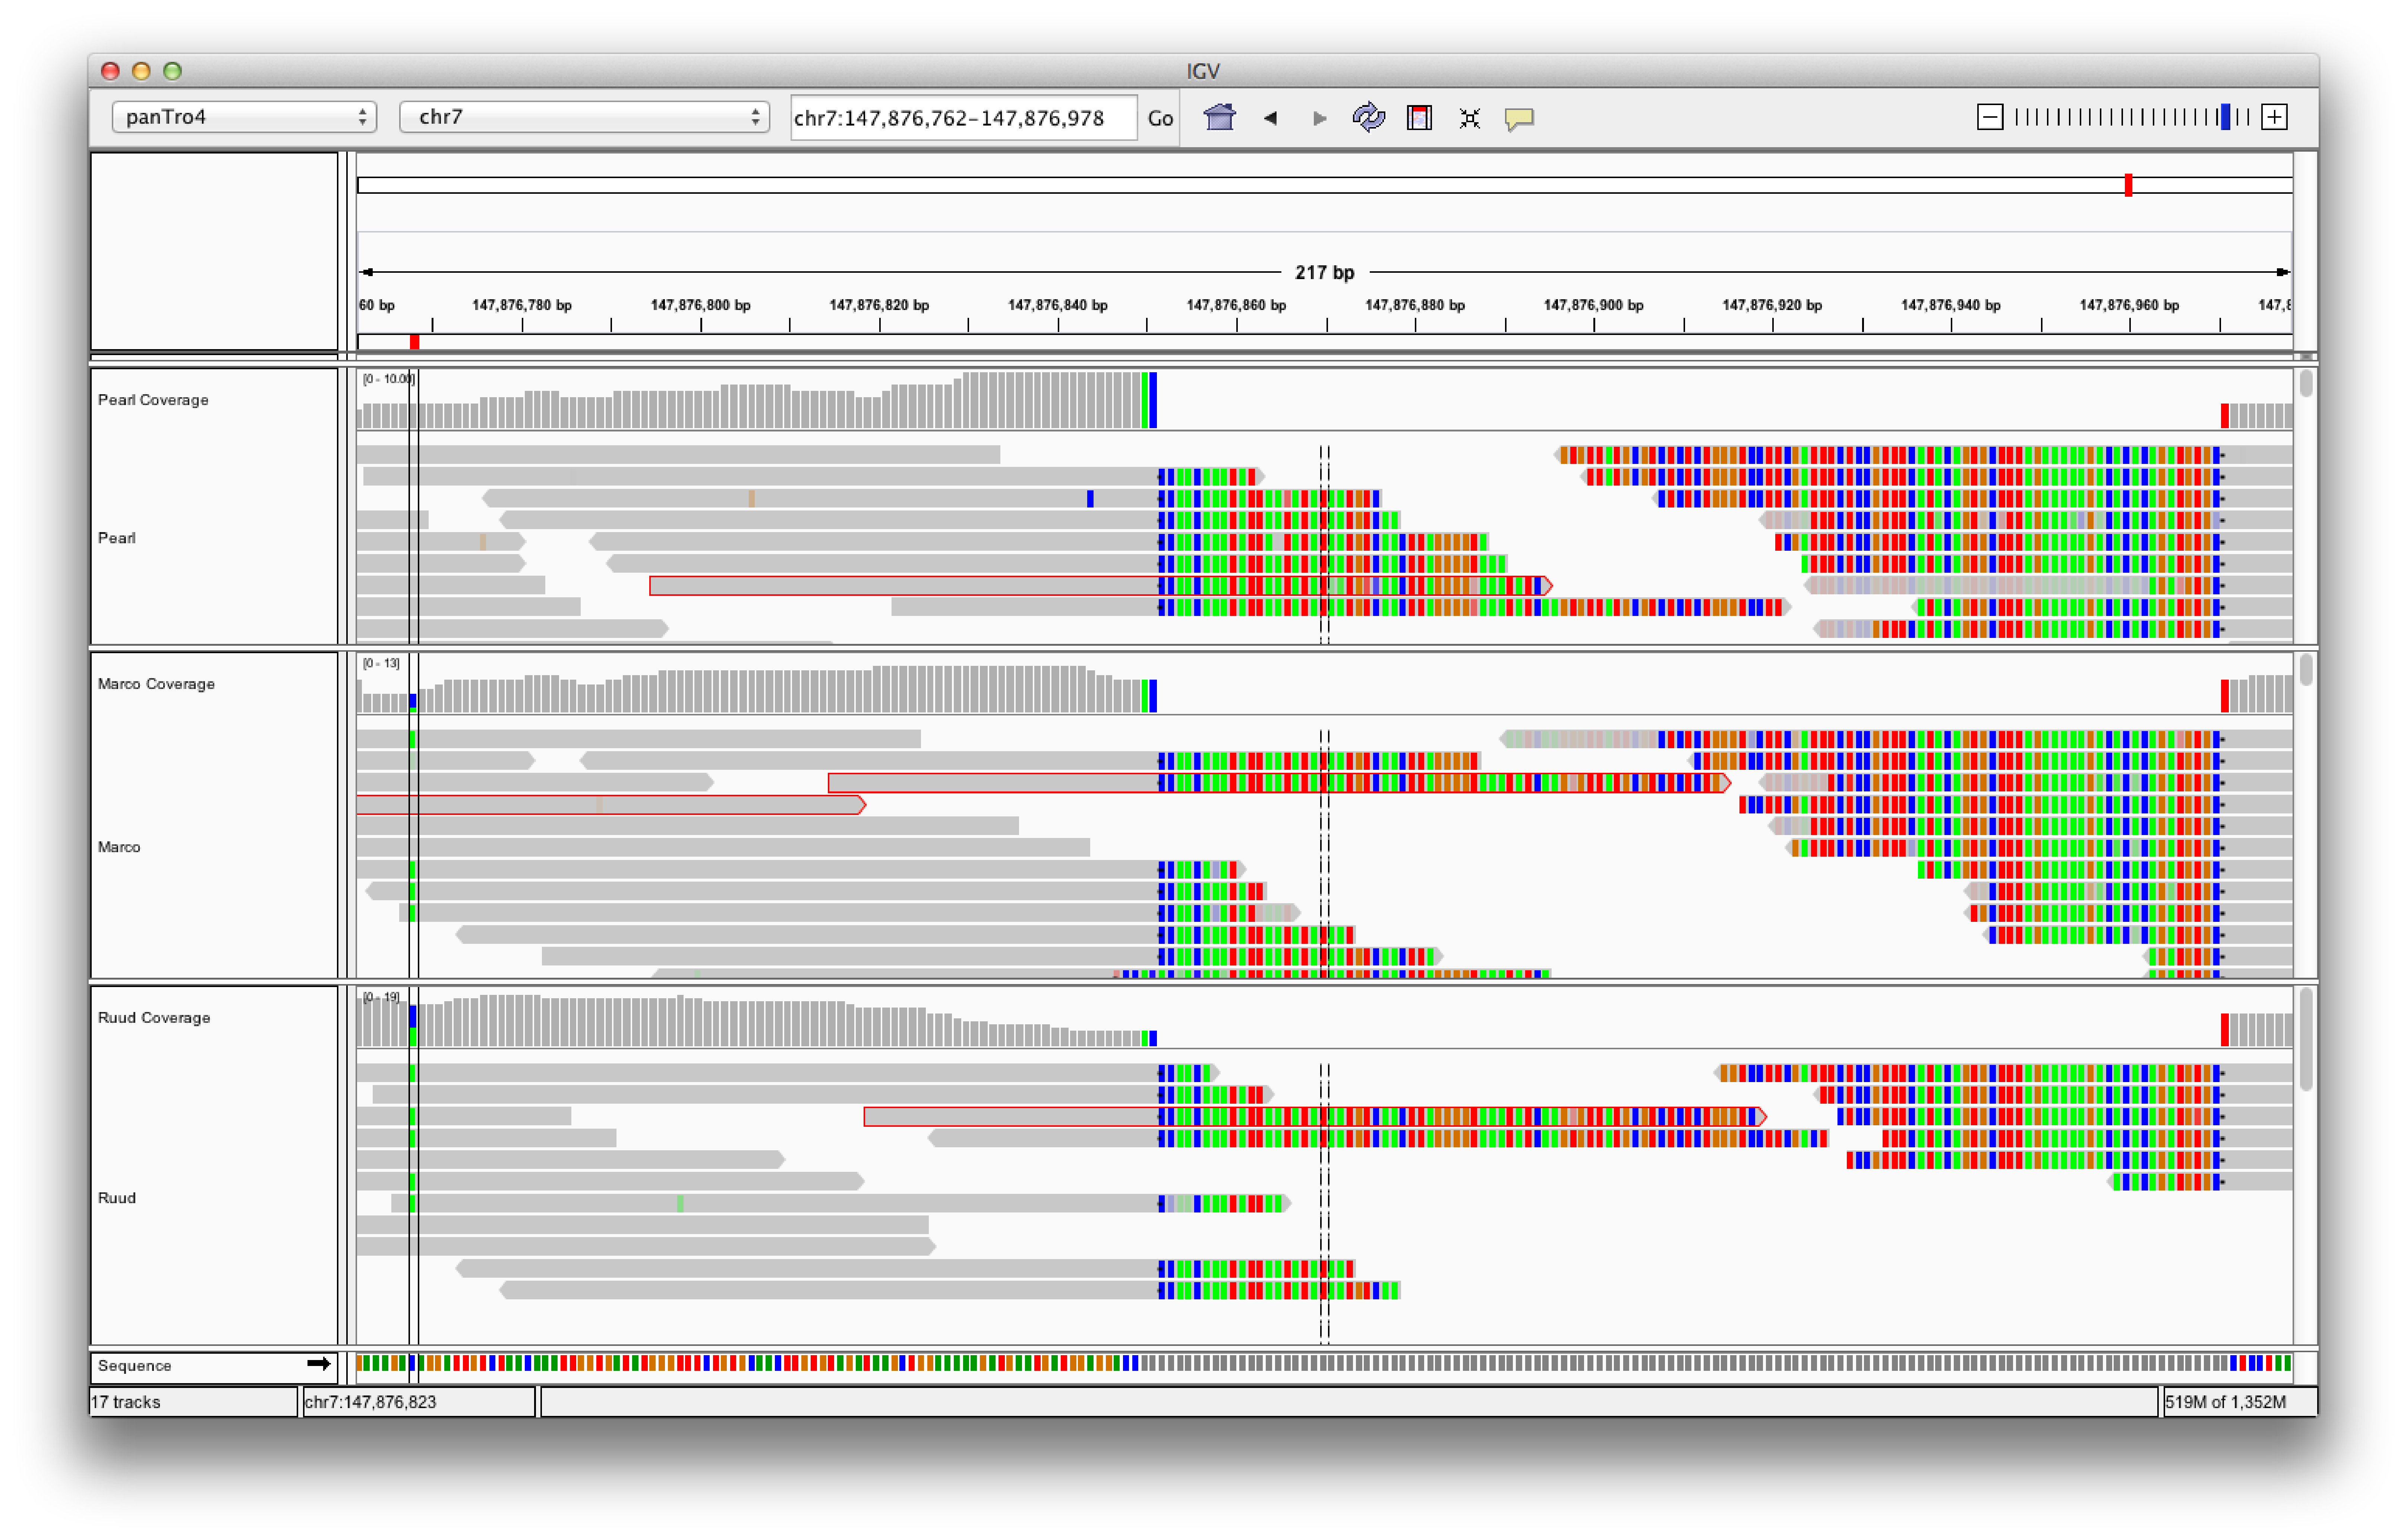
\includegraphics[width=0.9\textwidth]{refhole}
%  \caption{Read coverage near the aberrant \textit{de novo} SNV and a reference assembly gap in chimpanzee pedigree founders, Pearl and Marco (top and middle tracks, respectively) and F1 progeny, Ruud (bottom track).}
%  \label{fig:refhole}
%\end{figure}

To guard against these false calls, we imposed two conditions.  First, we required that no kmer in the alternate branch have edges present in the parental colors of the dirty graph but absent in the clean graph.  Effectively, the absense of an edge is only to be trusted if it is never observed in the raw data.  Second, we required that a DNM contain at least $24$ novel kmers.  This cutoff is fairly arbitrary, chosen by simply considering that for graphs constructed at $k=47$, this is $(k+1)/2 = 24$ kmers, or a little more than half of the kmers generated by a single SNP being novel.  This ensures that our calls reach some reasonable quality threshold before we consider them.

\section{\textit{De novo} mutations in the \textit{P. troglodytes} dataset}

\begin{figure}[h!]
  \centering
    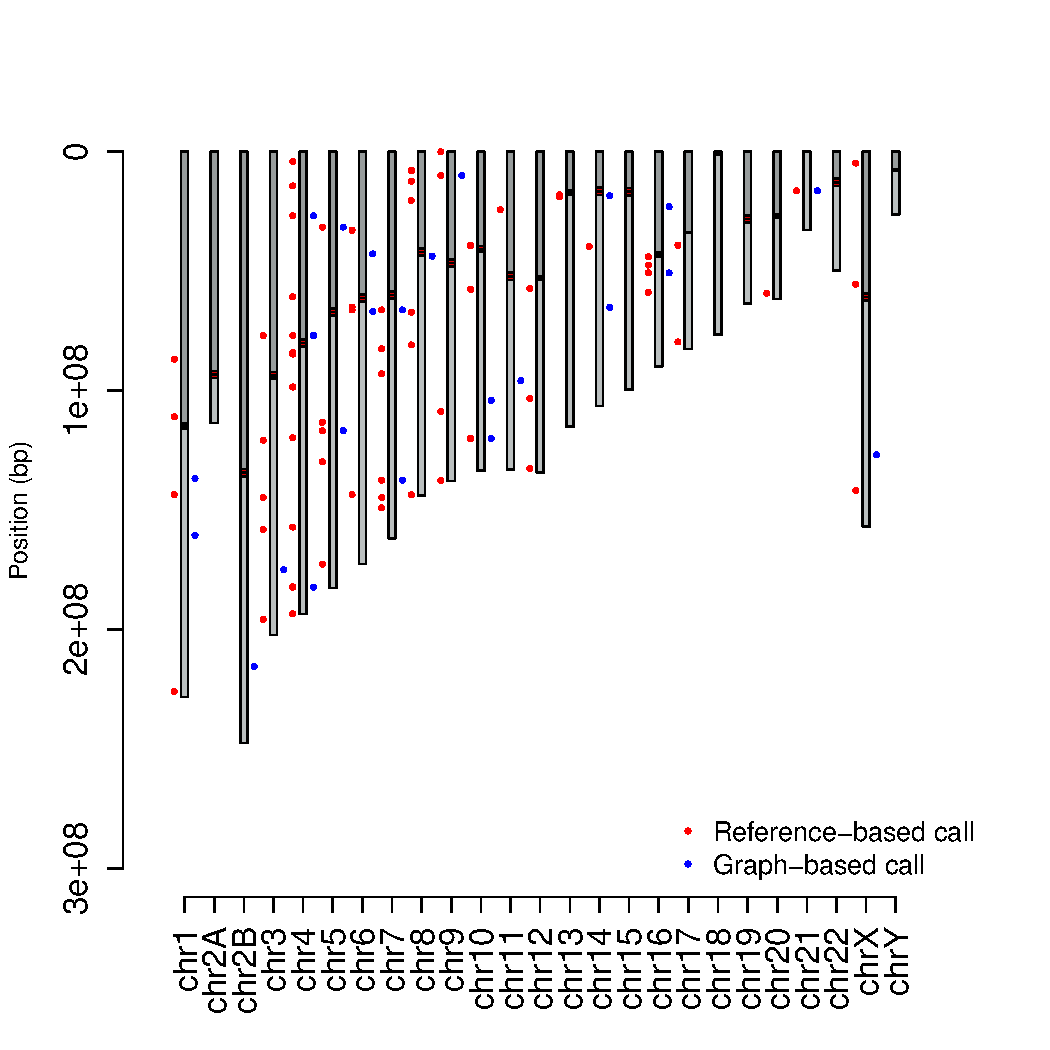
\includegraphics[width=0.95\textwidth]{ideogram-1}
  \caption{Positions of \textit{de novo} mutations from the reference-based analysis (left of ideogram) and graph-based analysis (graph-based analysis).}
  \label{fig:ideogram-1}
\end{figure}

We produced graph-based DNM calls using our software in three samples: Dennis, Ruud, and Marlies.  We have listed all variant calls made in both the reference-based and graph-based analyses in Table \ref{ruud_rf_vs_graph}, itself an expansion of a Table $S6$ in the Supplementary Online Methods from Venn \textit{et al.}, 2014\cite{Venn:2014ep}.  Each row in the table lists a variant call made in the sample.  Each call is either unique to the reference-based analysis (in which case the GraphCall column is "."), or the graph-based analysis (in which case the NovelKmerFound column is "novel"), or both (NovelKmerFound is "present" and GraphCall indicates the event type).  Many of the reference-based calls were validated by Sequenom assays.  Validation status is indicated as $1$ (validated), $0$ (failed to validate), or $-$ (not validated).  For brevity, we have only included the results for Ruud in this listing, as this sample had the largest number of validated sites.

We considered sites that passed validation and others that passed visual inspect of alignments in IGV to be true positives.  $31$ such sites were recovered in the graphical analysis.  $19$ were classified as false negatives - that is, present in the reference-based analysis and seemingly real, but missed by our caller.  The positions of each DNM are shown in Figure \ref{fig:ideogram-1}, with variants from the reference-based analysis to the left of the ideogram and variants from the graph-based analysis to the right.

The reason for the missed variants is clear: in all cases, the some ($8$) or all ($11$) of the novel kmers needed to seed the traversal were missing.  Often, the novel kmers were found in the graph at coverage $< 4$, the automatically determined coverage threshold applied by McCortex.  This problem of missing sites is much more pronounced in Marlies.  While we recover $3$ of the known and validated DNMs, we fail to recover $23$; each one of these is missing a novel kmer somewhere along the variant branch, preventing traversal.  All but two sites have novel kmers present in the dirty graph of the child at coverages less than the automatically determined cut-off of $6$.  Dennis is affected most profoundly; with a coverage threshold of $8$, we recover $4$ sites and miss $50$.

\section{Summary}

Despite incomplete recovery of the known DNM repertoire, the results in Ruud, Marlies, and Dennis demonstrate that a reference-free, graph-based approach to DNM discovery does successfully find true \textit{de novo} variation in a genome two orders of magnitude larger than it was designed for, in a diploid rather than haploid genome, and where coverage is substantially lower.  Interestingly enough, the failure to re-discover many sites is not due to our algorithm, but overaggressive cleaning thresholds chosen by the assembly software.  False positives are not the problem; sensitivity is the primary concern in low coverage data, especially when the presence of heterozygotes halves the coverage available to construct the graph and make the call.

Most assembly algorithms are not written to discover heterozygous sites, but rather to produce the best draft assembly possible.  When contig length is considered the metric of measuring "best", it is no surprise that nearly every assembler makes a choice to drop heterozygous sites from the graph, randomly choosing one allele or another.  The graph structure we manipulate is automatically cleaned with this goal in mind.  Nearly every site we missed could have been recovered had the graph been cleaned at lower thresholds.  One wonders if a probabilistic approach to graph construction (wherein kmers and/or edges are assigned quality scores) would enable their recovery while keeping graph traversal tractable.  One also wonders if graphs need be cleaned at all if such a probabilistic construction were to exist.

% Please add the following required packages to your document preamble:
% \usepackage{booktabs}
\begin{landscape}
\begin{table}[]
\tiny
\centering
\caption{Variants found in $F_1$ sample, Ruud, in the reference-based and graph-based analyses.}
\label{tbl:ruud_ref_vs_graph}
\begin{tabular}{@{}lllllllll@{}}
\toprule
Chr   & Pos       & NovelKmer                                                & NovelKmerFound     & GraphCall & Allele0  & Allele1             & Validated & Status \\ \midrule
chr1  & 143564354 & \texttt{AAGATTCAGGACCTTGGGGAGAGCACTTATTAATGGAAGCTATAGAT} & missing            & .         & T        & C                   & 1         & FN     \\
chr1  & 130945113 & \texttt{CCACGCAAGTTAGAAGCATCTGATAGTGGAGATTTGAGGGTTGGGGC} & missing            & .         & A        & G                   & 1         & FN     \\
chr1  & 2700783   & \texttt{GGCTTACGTCCGGGGCGGTCCAGCGTGCCCAGGAGCCGGCGAGCTCT} & present            & .         & C        & T                   & 0         & FN     \\
chr1  & 136785165 & \texttt{TGTTGATTCAGATGAGAGTTTCTATATCAAGGCAGCTTCCCTCTCAT} & present            & SNP       & C        & A                   & 1         & TP     \\
chr1  & 160615945 & \texttt{ATGGTCTTTTCAAAGAATAGACATGCTTACTGTTCAATATAGGCAAA} & novel              & SNP       & G        & A                   & -         & TP     \\
chr2A & 18269979  & \texttt{AAAAGATATGAAATTATTCATCTAGATAAGTTTCAGGACAGCCATCT} & present;not\_novel & .         & G        & A                   & 1         & FN     \\
chr2A & 12036323  & \texttt{AATGCAGTGGCACGGTCTCAGCTCAATGCAACCTCCACCTCCCGGGT} & missing            & .         & C        & A                   & 1         & FN     \\
chr2A & 27752205  & \texttt{CCTGATGAAAAGGAACTCCCTTCACCAGCAGATTTCCCCACTTCCTC} & missing            & .         & T        & C                   & 1         & FN     \\
chr2B & 154740624 & \texttt{ACTAGATTAGCTAGATACAGAGTGTTGATTGGTGTATTTACAAACTC} & missing            & .         & CC       & TG                  & 0         & FP     \\
chr2B & 154740632 & \texttt{AGCTAGATACAGAGTGTCCATTGGTATAATTACAAACTCTGAGCTAG} & missing            & .         & GTAT     & ATAA                & 0         & FP     \\
chr2B & 127429405 & \texttt{GAGGAGGCTATGTGGTCAATGGAGTGTTATCTTAGTTCCATCTTACA} & present            & SNP       & T        & G                   & 1         & TP     \\
chr2B & 155669031 & \texttt{TCTGATCTACACTCATCTGAAGAAATGAATACCAAAATGAAAAATTA} & missing            & .         & C        & T                   & 1         & FN     \\
chr2B & 215527935 & \texttt{CATCTTTTTTTGCTTTTTTGTCAATAACTAAATATCAATTTAATCAA} & novel              & MNP       & TGTTAGTG & AATTTAATCAAATTTAAAT & -         & TP     \\
chr3  & 16093871  & \texttt{GGGAGGGCTGCACATGGCTTGAACTTGTAAGTTCAAGGCCAGCCTGG} & present            & SNP       & C        & T                   & 0         & TP     \\
chr3  & 189709073 & \texttt{GTGCTTGTAGTCCCAGTTATTGAGGCGGCTGAGGTGGGAGGATTGCT} & present            & .         & A        & C                   & 1         & FN     \\
chr3  & 175043577 & \texttt{TAAGCTTCACCTACAGAAATTCAGTGAGACAGAAATAGGAATTCAGT} & present            & SNP       & A        & G                   & 1         & TP     \\
chr3  & 158138958 & \texttt{TCTTGATCCACAATCAACGGTTTGGCTAGAAACATGAAGGATAACTT} & present            & .         & A        & C                   & 1         & FN     \\
chr4  & 76952784  & \texttt{AACTGTGGGTTTGCATGATTCATTCAAAAACATCATTTGGGGGTCGT} & present            & SNP       & G        & A                   & 1         & TP     \\
chr4  & 84732820  & \texttt{AATTTCCAGAGGAGGAAGAAAGAGACGGAATTCTAAGCACAGCGGGC} & present            & SNP       & T        & C                   & 1         & TP     \\
chr4  & 182283692 & \texttt{CAACTTTCAGATATATTTGTTATACTGTTTTCACATAGCTCTATATT} & present            & SNP       & C        & T                   & 1         & TP     \\
chr4  & 98504146  & \texttt{CTTCAAACAGCTAGGAATTAATCAGACAGCTTGGCTTCAAGCTCGGT} & missing            & .         & C        & A                   & 0         & FP     \\
chr4  & 182152047 & \texttt{GGCATGATTTGGCAGCGGCTGGTACTGCTTGTTCCTTTCCATGTTTA} & present            & .         & C        & T                   & 0         & FN     \\
chr4  & 26839240  & \texttt{GTGTATGACTAGTGCTTTCTTTTATAATTCTATTTGTAAATGTTATG} & present            & SNP       & G        & A                   & 1         & TP     \\
chr4  & 119767460 & \texttt{TAAGCCACCACTCCTGGCCTTGGAACGATTTTAACAAGACAAATGTG} & present            & SNP       & T        & C                   & 0         & TP     \\
chr4  & 14340935  & \texttt{TCAGTGCTAGAAAATGTTTGGGTGTTGACCAGCCTGAGTAACAAGTA} & present            & SNP       & C        & T                   & 1         & TP     \\
chr5  & 31583344  & \texttt{AGTGTTGGGGCAGGGGAGGGGGGAGGAAAAGGGAGTTTACAAAAAGA} & present            & SNP       & A        & G                   & 1         & TP     \\
chr5  & 113309277 & \texttt{GAAGTGAATCTGATAGATCAGAAAGGCCTGTATTAGTACGCCAGTCA} & present            & .         & A        & G                   & 1         & FN     \\
chr5  & 116781586 & \texttt{GTTAAAAAAGCTTCAAATAATCATACTCAAAACCTCTTAACTTGCTG} & present            & SNP       & T        & C                   & 1         & TP     \\
chr5  & 129805166 & \texttt{TGAAAAGAGTCTTATTTCCCTTTCATTTATGAAGCTTAGTTTGGCTA} & present            & SNP       & C        & T                   & 1         & TP     \\
chr5  & 30381378  & \texttt{TGTATTTACCCAATGCCTGTGCCCCTGTTGTAGACAAGAAGTAACTA} & present            & SNP       & C        & T                   & 0         & TP     \\
chr6  & 14157189  & \texttt{CCCACAAAAATAACTAGGGGATAATATGAGGGTGGACTTAGTTCTAG} & present            & SNP       & T        & A                   & 1         & TP     \\
chr6  & 42794716  & \texttt{TAAGCCCTGGCATGTCAAGTGTGCATGCATACACACACACCTGCTGC} & present            & SNP       & C        & T                   & 1         & TP     \\
chr6  & 66924441  & \texttt{ATGTTAGTAGCAGCAGCATTTCTTTGTTCTCAAAACATCACAAAAAC} & novel              & SNP       & T        & C                   & -         & NA     \\
chr7  & 137493791 & \texttt{ATAAAATAAAATAATAACAGAGTACATGTAACTATATATAGAAATAC} & present            & SNP       & G        & A                   & 0         & TP     \\
chr7  & 82509177  & \texttt{CATTTAACTTAGCAAAGAAAATCTATATAATTGAGACTAAAATACAT} & missing            & .         & G        & T                   & 0         & FP     \\
chr7  & 144765721 & \texttt{CCATGGTGGTTAATAGAGCTCATTAATACATCTAAGTATTACTAAAT} & missing            & .         & C        & A                   & 1         & FN     \\
chr7  & 66260437  & \texttt{GCGTATTGCACGGGAATGTGTTTAACTGTCAGCAGAGGTGGCCTGGA} & present            & SNP       & G        & C                   & 1         & TP     \\
chr8  & 43737875  & \texttt{AGAACGGTTTTGAAACACTCTTTTTGTAGAATGTGTAAGTGAAAACT} & novel              & SNP       & A        & G                   & -         & NA     \\
chr8  & 43738841  & \texttt{AGAGTGTTTCAAAACTGCTGTATGAAAAGGAATGTTCAACGCTGTGA} & novel              & SNP       & G        & A                   & -         & NA     \\
chr8  & 43738841  & \texttt{AGAGTGTTTCAAAACTGCTGTATGAAAAGGAATGTTCAACGCTGTGA} & novel              & SNP       & T        & G                   & -         & NA     \\
chr9  & 110484253 & \texttt{CCAACCAACTTGCTGTATACACCTTAGACAAGTCATTTGACCTTTCA} & present            & SNP       & G        & A                   & 1         & TP     \\
chr9  & 9965284   & \texttt{TTGGGAACAAAAAAGAGAGACTAGATGTCAGTATTAATTATAAAACT} & present            & SNP       & C        & T                   & 1         & TP     \\
chr10 & 120057414 & \texttt{TCAGTCACATAAAAATGTAGAGCAGACTGTTTGCAGTCTCCTTTAGG} & present            & SNP       & G        & A                   & 1         & TP     \\
chr10 & 80306438  & \texttt{TGTTGACCGGAAGCCTTACCAATAATATATAGTCGATTAACACATAT} & present            & SNP       & C        & T                   & 1         & TP     \\
chr10 & 57652821  & \texttt{TTCAAGGTCATCATATGAGACTAGCCTTATTATATCTATTTCACCTA} & present            & .         & A        & C                   & 1         & FN     \\
chr10 & 104106966 & \texttt{ATGCCTCTAATTGTTTATATTTATAAATATACTTATCAATACATTTA} & novel              & SNP       & A        & T                   & -         & TP     \\
chr11 & 24359728  & \texttt{ATTTTGAAATATCCATCTACAACTGTATTTGTTTTTGTTATTTTAAC} & missing            & .         & C        & T                   & 1         & FN     \\
chr11 & 95890315  & \texttt{ATGTCCTACAATCACATAGATTTTGCAATATAAACTTATATTGAATC} & novel              & SNP       & G        & A                   & -         & TP     \\
chr13 & 95270772  & \texttt{GCCCTGCAGCATGCCATTTTCTGGGCGTACAGAGACGAATATAAAAT} & missing            & .         & G        & C                   & 1         & FN     \\
chr14 & 39651670  & \texttt{ACACTCTAAGCATTAGACTTTGCATTGATAATATATATAAAATATAT} & present            & .         & C        & T                   & 0         & FN     \\
chr14 & 65139282  & \texttt{ACCACACTGCCTCCAAGGGAACTGATGCATACATTGCAGGCTTTGTG} & present            & SNP       & C        & T                   & 1         & TP     \\
chr14 & 18496753  & \texttt{ACAGATAAATAAATTTTAGAGACTGAAGAACCCACTTACATTCTCAA} & novel              & SNP       & A        & G                   & -         & TP     \\
chr15 & 91802628  & \texttt{AGAGCCTTTCTTGGAGAAGGAAAAGTGTTTTCACAGTCCAGCTATAA} & missing            & .         & C        & T                   & 1         & FN     \\
chr16 & 50735389  & \texttt{AATGAGCCTCAGCACGCAGCAGCCCTGACATCAAACGCACTTGTGTT} & present            & SNP       & C        & T                   & 1         & TP     \\
chr16 & 23062470  & \texttt{CCTTCTCATAGGTATGCTTTATGTTTCTGTAGAATTTTGGGATGAAG} & novel              & SNP       & C        & T                   & -         & NA     \\
chr19 & 3715608   & \texttt{GAGCCTTCCCTGAAATACTGCTCAGAGTCAAAACCGGGATCCCCGTT} & missing            & .         & G        & A                   & 1         & FN     \\
chr21 & 16410630  & \texttt{CAATGGATAGCATTTCATTAGATGGGAATGTGGTTCAAAGCTACCCA} & novel              & SNP       & G        & T                   & -         & TP     \\
chrX  & 9149290   & \texttt{CAAATATCCATCCAACTGAATACTCTCAAGGGATAGAAAGAAAAGAA} & missing            & .         & C        & T                   & 0         & FN     \\
chrX  & 126947832 & \texttt{GTCTAAGGAAGTCAGGCGCCAATTTCAATCATAAACATTTAAGAAAT} & present            & SNP       & T        & C                   & 0         & TP     \\ \bottomrule
\end{tabular}
\end{table}
\end{landscape}

